\documentclass[aspectratio=169,xcolor=table]{beamer}
\usepackage{tikz}
\usetikzlibrary{shapes,arrows,positioning,fit,calc,backgrounds}
\usepackage{listings}
% xcolor with table option loaded via documentclass
\usepackage{booktabs}

% Theme - Simple, no shadows
\usetheme{default}
\usecolortheme{default}
\setbeamertemplate{navigation symbols}{}
\setbeamertemplate{footline}[frame number]

% Reduce spacing to prevent content cutoff
\setbeamersize{text margin left=5mm,text margin right=5mm}
\setlength{\parskip}{0.3em}
\setlength{\itemsep}{0.2em}

% Colors
\definecolor{picolor}{RGB}{46,139,87}
\definecolor{awscolor}{RGB}{255,140,0}
\definecolor{browsercolor}{RGB}{70,130,180}

% Title
\title{Distributed AI-Powered Argument Analysis System}
\subtitle{Real-Time Emotion Classification and Multi-Source Fact-Checking}
\author{Ifesi Onubogu}
\institute{AIoT Project}
\date{\today}

\begin{document}

% ====================
% TITLE SLIDE
% ====================
\begin{frame}
\titlepage
\end{frame}

% ====================
% OUTLINE
% ====================
\begin{frame}{Outline}
\tableofcontents
\end{frame}

% ====================
% SECTION 1: OVERVIEW
% ====================
\section{Project Overview}

\begin{frame}{Problem Statement}
\begin{block}{Challenge}
In an era of increasing polarization and misinformation, how do we:
\begin{itemize}
    \item Analyze emotional dynamics in real-time conversations?
    \item Verify factual claims against authoritative sources?
    \item Present crowd-sourced predictions for subjective statements?
\end{itemize}
\end{block}

\vspace{0.5cm}

\begin{block}{Solution}
A distributed edge-cloud system that:
\begin{itemize}
    \item Captures and processes conversations on Raspberry Pi
    \item Analyzes emotions using fine-tuned transformers on AWS
    \item Fact-checks claims via RAG, Polymarket, and web search
    \item Visualizes results in interactive web interface
\end{itemize}
\end{block}
\end{frame}

\begin{frame}{Key Contributions}
\begin{enumerate}
    \item \textbf{Hybrid Fact-Checking Pipeline}
    \begin{itemize}
        \item First system to combine curated knowledge base (RAG), prediction markets, and web search
    \end{itemize}

    \vspace{0.3cm}

    \item \textbf{Segment-Level Emotion Analysis}
    \begin{itemize}
        \item Per-utterance emotion classification (73.2\% accuracy)
        \item 8 emotion classes optimized for argument detection
    \end{itemize}

    \vspace{0.3cm}

    \item \textbf{LRU-Cached Market Discovery}
    \begin{itemize}
        \item Dynamic cache management for prediction market links
        \item API fallback for unseen topics
    \end{itemize}

    \vspace{0.3cm}

    \item \textbf{Privacy-Preserving Edge Architecture}
    \begin{itemize}
        \item Local processing on Raspberry Pi
        \item Cloud inference only for heavy models
    \end{itemize}
\end{enumerate}
\end{frame}

% ====================
% SECTION 2: ARCHITECTURE
% ====================
\section{System Architecture}

\begin{frame}{High-Level Architecture}
\begin{center}
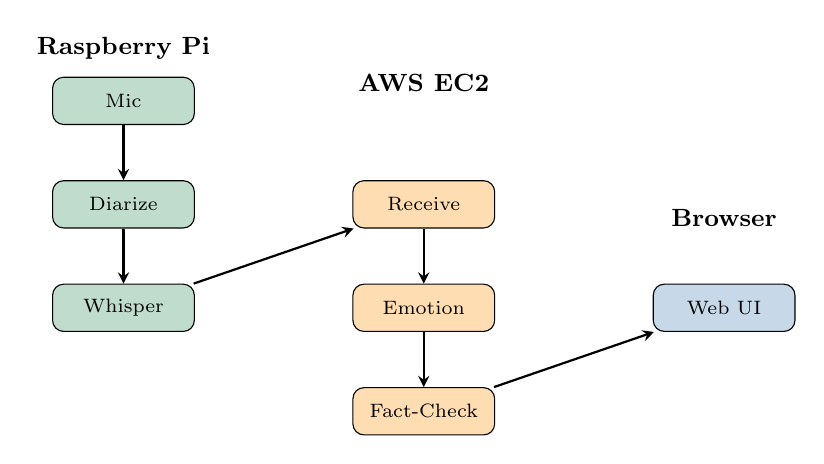
\begin{tikzpicture}[
    node distance=0.7cm and 2cm,
    box/.style={rectangle, draw, rounded corners, minimum height=0.6cm, minimum width=1.8cm, align=center, font=\scriptsize},
    arrow/.style={->, thick, >=stealth}
]

% Raspberry Pi
\node[box, fill=picolor!30] (pi1) {Mic};
\node[box, fill=picolor!30, below=of pi1] (pi2) {Diarize};
\node[box, fill=picolor!30, below=of pi2] (pi3) {Whisper};
\node[above=0.1cm of pi1, font=\small\bfseries] {Raspberry Pi};

% AWS
\node[box, fill=awscolor!30, right=of pi2] (aws1) {Receive};
\node[box, fill=awscolor!30, below=of aws1] (aws2) {Emotion};
\node[box, fill=awscolor!30, below=of aws2] (aws3) {Fact-Check};
\node[above=1cm of aws1, font=\small\bfseries] {AWS EC2};

% Browser
\node[box, fill=browsercolor!30, right=of aws2] (br) {Web UI};
\node[above=0.6cm of br, font=\small\bfseries] {Browser};

% Arrows
\draw[arrow] (pi1) -- (pi2);
\draw[arrow] (pi2) -- (pi3);
\draw[arrow] (pi3) -- (aws1);
\draw[arrow] (aws1) -- (aws2);
\draw[arrow] (aws2) -- (aws3);
\draw[arrow] (aws3) -- (br);

\end{tikzpicture}
\end{center}

\vspace{0.2cm}
\begin{center}
\small\textbf{Edge} $\rightarrow$ \textbf{Cloud} $\rightarrow$ \textbf{Client}
\end{center}
\end{frame}

\begin{frame}{System Data Flow}
\begin{table}
\centering
\footnotesize
\begin{tabular}{clp{6cm}}
\toprule
\textbf{Step} & \textbf{Component} & \textbf{Action} \\
\midrule
\multicolumn{3}{l}{\cellcolor{blue!20}\textbf{Raspberry Pi (Edge) - 4-6 sec}} \\
1 & Microphone & Capture 30-second audio \\
2 & pyannote & Speaker diarization \\
3 & Whisper & Speech-to-text \\
4 & HTTP & POST to AWS \\
\midrule
\multicolumn{3}{l}{\cellcolor{orange!20}\textbf{AWS EC2 (Cloud) - 2-3 sec}} \\
5 & FastAPI & Receive files \\
6 & Emotion Model & Classify per segment \\
7 & Fact Checker & RAG + Polymarket + Web \\
8 & Database & Store results \\
\midrule
\multicolumn{3}{l}{\cellcolor{green!20}\textbf{Browser (Client) - <1 sec}} \\
9 & Gradio & Load web UI \\
10 & Visualization & Display analysis \\
\bottomrule
\end{tabular}
\end{table}

\vspace{0.1cm}
\begin{center}
\textbf{Total Latency:} 6-10 seconds end-to-end
\end{center}
\end{frame}


\begin{frame}{What Runs Where?}
\begin{columns}[T]

\column{0.33\textwidth}
\begin{block}{Raspberry Pi}
\small
\textbf{HW:} Pi 4 (4GB) + USB Mic

\vspace{0.1cm}
\textbf{Tasks:}
\begin{itemize}
    \item Audio capture
    \item Diarization
    \item Whisper STT
\end{itemize}
\end{block}

\column{0.33\textwidth}
\begin{block}{AWS EC2}
\small
\textbf{HW:} t2.large (2 vCPU, 8GB)

\vspace{0.1cm}
\textbf{Tasks:}
\begin{itemize}
    \item Emotion classification
    \item RAG + Polymarket
    \item Web search
    \item Storage
\end{itemize}
\end{block}

\column{0.33\textwidth}
\begin{block}{Browser}
\small
\textbf{UI:} Gradio web app

\vspace{0.1cm}
\textbf{Features:}
\begin{itemize}
    \item Chat bubbles
    \item Emotion badges
    \item Hover panels
    \item Source links
\end{itemize}
\end{block}

\end{columns}
\end{frame}

% ====================
% SECTION 3: EMOTION CLASSIFIER
% ====================
\section{Emotion Classification}

\begin{frame}{Emotion Classifier Architecture}
\begin{center}
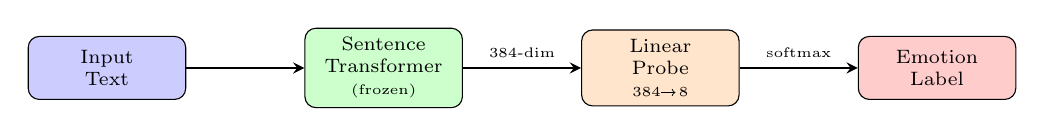
\begin{tikzpicture}[
    node distance=1.5cm,
    box/.style={rectangle, draw, rounded corners, minimum height=0.8cm, minimum width=2cm, align=center, font=\scriptsize},
    arrow/.style={->, thick, >=stealth}
]

\node[box, fill=blue!20] (input) {Input\\Text};
\node[box, fill=green!20, right=of input] (embed) {Sentence\\Transformer\\{\tiny (frozen)}};
\node[box, fill=orange!20, right=of embed] (probe) {Linear\\Probe\\{\tiny 384→8}};
\node[box, fill=red!20, right=of probe] (output) {Emotion\\Label};

\draw[arrow] (input) -- (embed);
\draw[arrow] (embed) -- node[above, font=\tiny] {384-dim} (probe);
\draw[arrow] (probe) -- node[above, font=\tiny] {softmax} (output);

\end{tikzpicture}
\end{center}

\vspace{0.3cm}

\begin{columns}[T]
\column{0.5\textwidth}
\textbf{Model:}
\begin{itemize}
    \item Pre-trained embedder (66M params frozen)
    \item 2-layer MLP (49K trainable)
    \item Fast inference (~100ms)
\end{itemize}

\column{0.5\textwidth}
\textbf{8 Emotion Classes:}
\begin{itemize}
    \item Calm, Confident, Defensive
    \item Dismissive, Passionate
    \item Frustrated, Angry, Sarcastic
\end{itemize}
\end{columns}
\end{frame}

\begin{frame}{Training Data Generation}
\begin{block}{Synthetic Data via GPT-4}
Generated 500 labeled examples using structured prompts for 8 emotion classes
\end{block}

\vspace{0.2cm}

\begin{columns}[T]
\column{0.5\textwidth}
\textbf{Prompt Structure:}
\begin{itemize}
    \item Specify topic \& emotion
    \item Include emotion patterns
    \item Generate 2-4 sentences
\end{itemize}

\vspace{0.2cm}

\textbf{Topics:}
\begin{itemize}
    \item Remote work, Climate
    \item EVs, Social media
    \item Healthcare, Politics
\end{itemize}

\column{0.5\textwidth}
\textbf{Example Patterns:}
\begin{itemize}
    \item Confident: "Obviously..."
    \item Defensive: "That's not fair..."
    \item Frustrated: "This is pointless..."
    \item Sarcastic: "Oh sure..."
\end{itemize}

\vspace{0.2cm}

\textbf{Data Split:}
\begin{itemize}
    \item Train: 400, Val: 100
    \item Balanced across 8 classes
\end{itemize}
\end{columns}
\end{frame}

\begin{frame}{Training Configuration}
\begin{columns}[T]

\column{0.5\textwidth}
\begin{block}{Hyperparameters}
\small
\begin{itemize}
    \item Adam optimizer, LR: 0.001
    \item Batch: 32, Epochs: 20
    \item Dropout: 0.3
    \item CrossEntropy loss
\end{itemize}
\end{block}

\column{0.5\textwidth}
\begin{block}{Why Linear Probe?}
\small
\begin{itemize}
    \item Only 49K trainable params
    \item Works with 400 examples
    \item Fast inference (~100ms)
    \item Low memory footprint
\end{itemize}
\end{block}

\end{columns}

\vspace{0.3cm}

\begin{center}
\textbf{Model:} 66M frozen + 49K trainable = 66M total params
\end{center}
\end{frame}

\begin{frame}{Testing Methodology}
\begin{block}{Test Setup}
\begin{itemize}
    \item 500 synthetic examples (GPT-4)
    \item Split: 400 train / 100 val
    \item 100 held-out test (balanced)
\end{itemize}
\end{block}

\vspace{0.2cm}

\begin{block}{Evaluation Process}
\begin{enumerate}
    \item Train 20 epochs, validate, select best
    \item Test on 100 held-out examples
    \item Real-world validation on recordings
\end{enumerate}
\end{block}

\vspace{0.2cm}

\begin{alertblock}{Note}
Synthetic data provides strong baseline for transfer learning
\end{alertblock}
\end{frame}

\begin{frame}{Emotion Classifier Results}
\begin{table}
\centering
\small
\begin{tabular}{lccc}
\toprule
\textbf{Metric} & \textbf{Mean} & \textbf{Std} & \textbf{Range} \\
\midrule
Accuracy & \textbf{73.2\%} & 4.1\% & 68-79\% \\
Precision & 71.8\% & 5.2\% & 64-78\% \\
Recall & 72.4\% & 4.8\% & 66-78\% \\
F1-Score & 72.1\% & 4.5\% & 66-78\% \\
\bottomrule
\end{tabular}
\end{table}

\vspace{0.3cm}

\begin{columns}[T]
\column{0.5\textwidth}
\textbf{Best Classes:}
\begin{itemize}
    \item Angry: 82\% F1
    \item Confident: 79\% F1
    \item Calm: 76\% F1
\end{itemize}

\column{0.5\textwidth}
\textbf{Challenging:}
\begin{itemize}
    \item Sarcastic: 65\% F1
    \item Defensive: 68\% F1
\end{itemize}
\end{columns}

\vspace{0.2cm}

\begin{alertblock}{Insight}
73\% for 8-way classification with only 400 examples!
\end{alertblock}
\end{frame}

% ====================
% SECTION 4: RAG SYSTEM
% ====================
\section{Fact-Checking with RAG}

\begin{frame}{Multi-Source Fact-Checking Pipeline}
\begin{center}
\begin{tikzpicture}[
    node distance=0.7cm and 1.5cm,
    box/.style={rectangle, draw, rounded corners, minimum height=0.6cm, minimum width=1.8cm, align=center, font=\tiny},
    arrow/.style={->, thick, >=stealth}
]

% Input
\node[box, fill=blue!20] (query) {Query};

% Three parallel sources
\node[box, fill=green!20, below left=1cm and 0.8cm of query] (kb) {📚 KB\\RAG};
\node[box, fill=purple!20, below=1cm of query] (poly) {📊 Polymarket\\Cache};
\node[box, fill=orange!20, below right=1cm and 0.8cm of query] (web) {🌐 Web\\DDG};

% Combine
\node[box, fill=red!20, below=2cm of query] (combine) {Aggregate};

% Output
\node[box, fill=yellow!20, below=of combine] (output) {Facts};

% Arrows
\draw[arrow] (query) -- (kb);
\draw[arrow] (query) -- (poly);
\draw[arrow] (query) -- (web);
\draw[arrow] (kb) -- (combine);
\draw[arrow] (poly) -- (combine);
\draw[arrow] (web) -- (combine);
\draw[arrow] (combine) -- (output);

\end{tikzpicture}
\end{center}

\vspace{0.2cm}
\small
\textbf{Three Sources:} 📚 Curated KB (semantic) | 📊 Polymarket (crowd opinion) | 🌐 Web (current news)
\end{frame}

\begin{frame}{Vector Database for Semantic Search}
\begin{block}{What is a Vector Database?}
Stores text as numerical vectors enabling similarity-based retrieval instead of keyword matching
\end{block}

\vspace{0.2cm}

\begin{columns}[T]
\column{0.5\textwidth}
\textbf{Keyword Search:}
\begin{itemize}
    \item Matches exact words only
    \item Misses synonyms
\end{itemize}
\textcolor{red}{$\times$ Limited by phrasing}

\column{0.5\textwidth}
\textbf{Semantic Search:}
\begin{itemize}
    \item Matches similar \textbf{meaning}
    \item Finds paraphrases
\end{itemize}
\textcolor{green}{$\checkmark$ Understands context}
\end{columns}

\vspace{0.3cm}

\begin{alertblock}{Our Implementation}
25 facts $\times$ 384 dimensions stored in memory for fast cosine similarity search
\end{alertblock}
\end{frame}

\begin{frame}{RAG: Vector Database Architecture}
\begin{center}
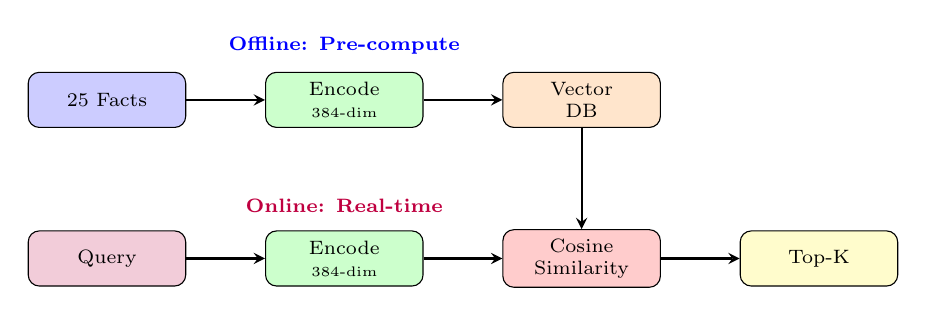
\begin{tikzpicture}[
    node distance=1cm,
    box/.style={rectangle, draw, rounded corners, minimum height=0.7cm, minimum width=2cm, align=center, font=\scriptsize},
    arrow/.style={->, thick, >=stealth}
]

% Offline indexing (top)
\node[box, fill=blue!20] (facts) {25 Facts};
\node[box, fill=green!20, right=of facts] (embed_offline) {Encode\\{\tiny 384-dim}};
\node[box, fill=orange!20, right=of embed_offline] (store) {Vector\\DB};
\draw[arrow] (facts) -- (embed_offline);
\draw[arrow] (embed_offline) -- (store);
\node[above=0.1cm of embed_offline, font=\scriptsize\bfseries\color{blue}] {Offline: Pre-compute};

% Online search (bottom)
\node[box, fill=purple!20, below=1.3cm of facts] (query) {Query};
\node[box, fill=green!20, right=of query] (embed_online) {Encode\\{\tiny 384-dim}};
\node[box, fill=red!20, right=of embed_online] (cosine) {Cosine\\Similarity};
\node[box, fill=yellow!20, right=of cosine] (topk) {Top-K};

\draw[arrow] (query) -- (embed_online);
\draw[arrow] (embed_online) -- (cosine);
\draw[arrow] (store.south) -- ++(0,-0.3) -| (cosine.north);
\draw[arrow] (cosine) -- (topk);
\node[above=0.1cm of embed_online, font=\scriptsize\bfseries\color{purple}] {Online: Real-time};

\end{tikzpicture}
\end{center}

\vspace{0.2cm}

\begin{itemize}
    \item \textbf{Model:} all-MiniLM-L6-v2, \textbf{Dimension:} 384
    \item \textbf{Metric:} Cosine similarity, \textbf{Threshold:} 0.3 (30\% match)
\end{itemize}
\end{frame}

\begin{frame}[fragile]{RAG: Knowledge Base Search}
\begin{block}{Semantic Search Algorithm}
\begin{lstlisting}[language=Python, basicstyle=\ttfamily\tiny, frame=single]
def search(query, top_k=3, threshold=0.3):
    # Encode query to 384-dim vector
    query_emb = model.encode(query)

    # Cosine similarity with all facts
    sims = cosine_similarity(query_emb, fact_embeddings)

    # Return top-k above threshold
    top_idx = argsort(sims)[-top_k:]
    return [facts[i] for i in top_idx if sims[i] >= threshold]
\end{lstlisting}
\end{block}

\vspace{0.2cm}
\textbf{Key Steps:} Encode query $\rightarrow$ Compute similarity $\rightarrow$ Filter by threshold $\rightarrow$ Return top matches
\end{frame}

\begin{frame}{Polymarket Integration with LRU Caching}
\begin{center}
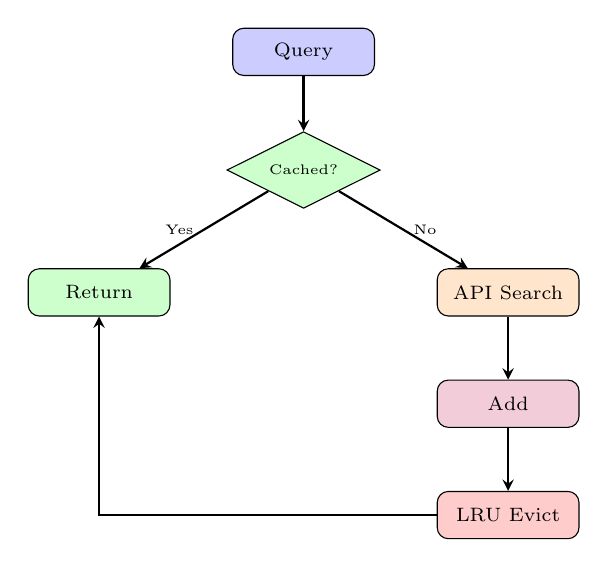
\begin{tikzpicture}[
    node distance=0.8cm,
    box/.style={rectangle, draw, rounded corners, minimum height=0.6cm, minimum width=1.8cm, align=center, font=\scriptsize},
    decision/.style={diamond, draw, fill=green!20, text width=1cm, align=center, aspect=2, font=\tiny},
    arrow/.style={->, thick, >=stealth}
]

\node[box, fill=blue!20] (query) {Query};
\node[decision, below=0.7cm of query] (cache) {Cached?};
\node[box, fill=green!20, below left=1cm and 1.2cm of cache] (return_cache) {Return};
\node[box, fill=orange!20, below right=1cm and 1.2cm of cache] (api) {API Search};
\node[box, fill=purple!20, below=of api] (add) {Add};
\node[box, fill=red!20, below=of add] (evict) {LRU Evict};

\draw[arrow] (query) -- (cache);
\draw[arrow] (cache) -- node[left, font=\tiny] {Yes} (return_cache);
\draw[arrow] (cache) -- node[right, font=\tiny] {No} (api);
\draw[arrow] (api) -- (add);
\draw[arrow] (add) -- (evict);
\draw[arrow] (evict) -| (return_cache);

\end{tikzpicture}
\end{center}

\vspace{0.2cm}

\begin{columns}[T]
\column{0.5\textwidth}
\textbf{Strategy:}
\begin{itemize}
    \item 22 preloaded markets
    \item Max 30 total, LRU eviction
\end{itemize}

\column{0.5\textwidth}
\textbf{Topics:}
\begin{itemize}
    \item Sports, Politics
    \item Culture, Tech, Finance
\end{itemize}
\end{columns}
\end{frame}

\begin{frame}{Web Search Integration}
\begin{center}
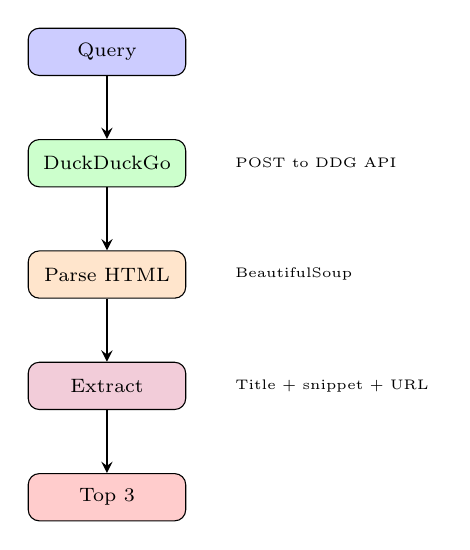
\begin{tikzpicture}[
    node distance=0.8cm,
    box/.style={rectangle, draw, rounded corners, minimum height=0.6cm, minimum width=2cm, align=center, font=\scriptsize},
    arrow/.style={->, thick, >=stealth}
]

\node[box, fill=blue!20] (query) {Query};
\node[box, fill=green!20, below=of query] (ddg) {DuckDuckGo};
\node[box, fill=orange!20, below=of ddg] (parse) {Parse HTML};
\node[box, fill=purple!20, below=of parse] (extract) {Extract};
\node[box, fill=red!20, below=of extract] (top3) {Top 3};

\draw[arrow] (query) -- (ddg);
\draw[arrow] (ddg) -- (parse);
\draw[arrow] (parse) -- (extract);
\draw[arrow] (extract) -- (top3);

% Compact annotations
\node[right=0.5cm of ddg, text width=2.5cm, font=\tiny] {POST to DDG API};
\node[right=0.5cm of parse, text width=2.5cm, font=\tiny] {BeautifulSoup};
\node[right=0.5cm of extract, text width=2.5cm, font=\tiny] {Title + snippet + URL};

\end{tikzpicture}
\end{center}

\vspace{0.2cm}

\begin{itemize}
    \item \textbf{Fallback} when KB/Polymarket lack info
    \item \textbf{Speed:} 1-2 sec, \textbf{Purpose:} Latest news
\end{itemize}
\end{frame}

% ====================
% SECTION 5: USE CASES
% ====================
\section{Use Cases}

\begin{frame}{Use Case 1: Corporate Decision-Making with Public Sentiment}
\begin{block}{Scenario}
Marketing team debating which F1 driver to approach for a brand partnership, based on public perception and championship momentum
\end{block}

\textbf{How System Helps:}
\begin{itemize}
    \item \textbf{Emotion Tracking:} Identifies when discussion becomes biased or emotionally charged
    \item \textbf{Fact-Checking:} Surfaces real-time public sentiment data from prediction markets
    \item \textbf{De-escalation:} Grounds debate in objective crowd-sourced probabilities
\end{itemize}

\vspace{0.3cm}

\begin{exampleblock}{Example: Max vs Lando F1 Championship Debate}
\textbf{Speaker A:} ``Max is the obvious choice -- everyone knows he'll win'' (Confident 82\%)\\
\textbf{Speaker B:} ``Lando has more momentum, the fans love him right now'' (Passionate 75\%)\\

\textbf{System shows:} Polymarket: Max 63\% vs Lando 28\% championship odds\\
Web: Recent fan sentiment analysis, social media engagement stats
\end{exampleblock}
\end{frame}

\begin{frame}{Use Case 2: Corporate Conflict Resolution}
\begin{block}{Scenario}
Team members disagreeing on project direction, resource allocation, or deadlines
\end{block}

\textbf{How System Helps:}
\begin{itemize}
    \item \textbf{Meeting Analysis:} Records team discussions, tracks emotional dynamics
    \item \textbf{Evidence-Based:} Provides market data, industry benchmarks, case studies
    \item \textbf{Post-Meeting Review:} Managers review conversation for missed concerns
\end{itemize}

\vspace{0.3cm}

\begin{exampleblock}{Example}
\textbf{Engineer:} "Everyone in the industry is moving to microservices" (Confident)\\

\textbf{System shows:} 📊 Polymarket: 55\% of companies still use monoliths\\
🌐 Recent survey: 40\% of microservice migrations failed\\
📚 Case study: When to choose monolith vs microservices
\end{exampleblock}
\end{frame}

\begin{frame}{Use Case 3: Educational Debate Analysis}
\begin{block}{Scenario}
Students debating controversial topics in classroom settings
\end{block}

\textbf{How System Helps:}
\begin{itemize}
    \item \textbf{Real-Time Feedback:} Students see emotion labels, learn self-awareness
    \item \textbf{Source Quality:} Distinguishes opinion claims from factual claims
    \item \textbf{Critical Thinking:} Teaches students to verify assertions with evidence
\end{itemize}

\vspace{0.3cm}

\begin{exampleblock}{Example}
\textbf{Student A:} "Most people think climate change is the biggest threat" (Passionate)\\

\textbf{System shows:} 📊 Polymarket: 68\% rate climate in top 3 global risks\\
📚 Pew Research: Public opinion varies by age and region\\
🌐 Latest IPCC report on climate consensus
\end{exampleblock}
\end{frame}

\begin{frame}{Use Case 4: Political Debate Fact-Checking}
\begin{block}{Scenario}
Live political debates, town halls, or campaign events
\end{block}

\textbf{How System Helps:}
\begin{itemize}
    \item \textbf{Real-Time Verification:} Fact-checks claims as candidates speak
    \item \textbf{Public Opinion:} Shows what voters actually think via prediction markets
    \item \textbf{Emotional Analysis:} Detects when candidates become defensive or evasive
\end{itemize}

\vspace{0.3cm}

\begin{exampleblock}{Example}
\textbf{Candidate:} "Everyone agrees my healthcare plan is the best solution" (Confident)\\

\textbf{System shows:} 📊 Polymarket: Plan has 45\% approval, 38\% disapproval\\
📚 CBO analysis: Plan would cost \$2.1T over 10 years\\
🌐 Kaiser poll: 52\% prefer alternative approach
\end{exampleblock}
\end{frame}

% ====================
% SECTION 6: RESULTS
% ====================
\section{Results \& Demo}

\begin{frame}{System Performance Metrics}
\begin{table}
\centering
\begin{tabular}{lcc}
\toprule
\textbf{Component} & \textbf{Metric} & \textbf{Value} \\
\midrule
\textbf{Raspberry Pi} & & \\
Speaker Diarization & Processing Time & 2-3 sec \\
Whisper Transcription & Processing Time & 2-3 sec \\
Total Pi Processing & Latency & 4-6 sec \\
\midrule
\textbf{AWS EC2} & & \\
Emotion Classifier & Accuracy & 73.2\% \\
Emotion Classifier & Inference Time & 100 ms \\
RAG Search & Query Time & 50 ms \\
Polymarket Lookup & Query Time & 80 ms \\
Web Search & Query Time & 1-2 sec \\
Total AWS Processing & Latency & 2-3 sec \\
\midrule
\textbf{End-to-End} & & \\
Total System Latency & Pi + AWS + Network & 6-10 sec \\
\bottomrule
\end{tabular}
\end{table}
\end{frame}

\begin{frame}{Interactive Visualization}
\begin{columns}[T]

\column{0.5\textwidth}
\textbf{Features:}
\begin{itemize}
    \item Color-coded speaker bubbles
    \item Emotion badges per segment
    \item Hover to see fact-checks
    \item KB + Polymarket + Web sources
\end{itemize}

\column{0.5\textwidth}
\begin{alertblock}{Live Demo}
\texttt{54.209.249.85:7863}
\end{alertblock}

\vspace{0.2cm}

\textbf{Example Output:}
\begin{itemize}
    \item Speaker emotions
    \item Supporting facts
    \item Contradicting claims
\end{itemize}

\end{columns}
\end{frame}

\begin{frame}{Live System Output}
\begin{center}
\includegraphics[width=0.9\textwidth,height=0.75\textheight,keepaspectratio]{ui_screenshot.png}
\end{center}

\vspace{0.2cm}
\begin{center}
\small
Real conversation analyzed showing emotion detection and web fact-checking sources
\end{center}
\end{frame}

\begin{frame}{System Output Examples}
\begin{columns}[T]

\column{0.48\textwidth}
\begin{center}
\textbf{Chat Conversation View}
\includegraphics[width=\textwidth,height=0.6\textheight,keepaspectratio]{s1.png}
\end{center}
\small Speaker segments with emotion labels

\column{0.48\textwidth}
\begin{center}
\textbf{Analysis Panel}
\includegraphics[width=\textwidth,height=0.6\textheight,keepaspectratio]{s2.png}
\end{center}
\small Emotion metrics + Polymarket predictions

\end{columns}
\end{frame}

% ====================
% SECTION 7: FUTURE WORK
% ====================
\section{Future Directions}

\begin{frame}{Future Work: Technical Improvements}
\begin{enumerate}
    \item \textbf{Real-Time Processing}
    \begin{itemize}
        \item Stream audio continuously instead of 30-second windows
        \item WebSocket connections for live emotion updates
        \item Reduce end-to-end latency to <3 seconds
    \end{itemize}

    \vspace{0.3cm}

    \item \textbf{Improved Emotion Classification}
    \begin{itemize}
        \item Fine-tune on real conversation data (not synthetic)
        \item Add audio features (pitch, volume, speaking rate)
        \item Multi-modal model combining text + audio
        \item Target 85\%+ accuracy
    \end{itemize}

    \vspace{0.3cm}

    \item \textbf{Enhanced Fact-Checking}
    \begin{itemize}
        \item Integrate scholarly databases (arXiv, PubMed)
        \item Add fact verification model (check claim truthfulness)
        \item Expand knowledge base to 1000+ curated facts
        \item Support multilingual fact-checking
    \end{itemize}
\end{enumerate}
\end{frame}

\begin{frame}{Future Work: New Features}
\begin{enumerate}
    \item \textbf{Argument Summarization}
    \begin{itemize}
        \item Generate concise summaries of key points
        \item Identify areas of agreement vs disagreement
        \item Extract action items and next steps
    \end{itemize}

    \vspace{0.3cm}

    \item \textbf{Bias Detection}
    \begin{itemize}
        \item Detect logical fallacies (ad hominem, straw man)
        \item Identify cognitive biases (confirmation bias, anchoring)
        \item Flag misleading statistics or cherry-picked data
    \end{itemize}

    \vspace{0.3cm}

    \item \textbf{Multi-Speaker Scaling}
    \begin{itemize}
        \item Support 3+ speakers in group discussions
        \item Track interruptions and speaking time balance
        \item Identify dominant speakers and quiet participants
    \end{itemize}
\end{enumerate}
\end{frame}

\begin{frame}{Future Work: Deployment \& Applications}
\begin{columns}[T]

\column{0.5\textwidth}
\textbf{Deployment:}
\begin{itemize}
    \item Mobile app for iOS/Android
    \item Zoom/Teams plugin for virtual meetings
    \item Smart speaker integration (Alexa, Google Home)
    \item Offline mode for privacy-sensitive contexts
\end{itemize}

\vspace{0.5cm}

\textbf{Privacy Enhancements:}
\begin{itemize}
    \item On-device emotion classification
    \item Differential privacy for stored data
    \item User consent and data deletion
    \item End-to-end encryption
\end{itemize}

\column{0.5\textwidth}
\textbf{New Applications:}
\begin{itemize}
    \item Mental health therapy sessions
    \item Customer service quality monitoring
    \item Podcast/media content analysis
    \item Diplomatic negotiations
    \item Legal mediation
\end{itemize}

\vspace{0.5cm}

\textbf{Research Directions:}
\begin{itemize}
    \item Causal analysis of de-escalation
    \item Longitudinal studies of conflict patterns
    \item Cross-cultural emotion detection
    \item Ethical guidelines for AI mediation
\end{itemize}

\end{columns}
\end{frame}

% ====================
% CONCLUSION
% ====================
\section{Conclusion}

\begin{frame}{Summary}
\begin{block}{What We Built}
A distributed edge-cloud system for real-time conversation analysis:
\begin{itemize}
    \item \textbf{73.2\%} emotion accuracy (8 classes)
    \item \textbf{3-source} fact-checking: RAG + Polymarket + Web
    \item \textbf{6-10 sec} end-to-end latency
\end{itemize}
\end{block}

\vspace{0.2cm}

\begin{block}{Key Innovations}
\begin{enumerate}
    \item Hybrid fact-checking with prediction markets
    \item LRU-cached market discovery
    \item Segment-level emotion analysis
    \item Privacy-preserving edge architecture
\end{enumerate}
\end{block}

\vspace{0.2cm}

\begin{alertblock}{Impact}
Reduces bias by providing objective facts and public opinion data
\end{alertblock}
\end{frame}

\begin{frame}{Thank You}
\begin{center}
\Huge Thank You!

\vspace{1cm}

\Large Questions?

\vspace{1cm}

\normalsize
\textbf{Project Links:}\\
\vspace{0.3cm}
GitHub: \texttt{github.com/ifesionubogu/aiot\_project}\\
Live Demo: \texttt{http://54.209.249.85:7863/}\\
Technical Report: See \texttt{TECHNICAL\_REPORT.pdf}

\end{center}
\end{frame}

\end{document}
